\chapter{Introduction}\label{ch:intro}

\section{Dual-Settlement Nodal Electricity Markets}\label{sec:dual-settlement-nodal-electricity-markets}

The increasing integration of renewable energy sources into the electrical grid has led to heightened volatility and
uncertainty in electricity prices.
This presents a major challenge for electricity market participants, who must be able
to accurately forecast electricity prices to make informed investment and trading decisions.
To address this challenge, the application of machine learning, and in particular deep generative models, to
day-ahead electricity price forecasting has become a topic of significant interest.

The North American electrical grid, sometimes regarded as the ``world's largest machine,'' is a feat of modern
engineering and operations that provides a critical resource for over 400 million individuals.
While the planning, construction, and maintenance of the physical infrastructure are non-trivial tasks,
post-completion the continuous and efficient operation of grid resources poses perhaps an even greater challenge.
To keep generation and demand synchronized, a grid operator must dispatch the least-cost optimal
generators such that all electrical loads are \textit{exactly} satisfied.
Furthermore, the matching must be done continuously despite uncertainty in the load, weather, generation,
grid topology, fuel prices, etc., lest there be a catastrophic failure in overall grid operations~\cite{ercotfail}.

The early grid was operated by local, vertically integrated utilities that owned all the generation and transmission in
an area.
Due to the small scale of the grids and relative certainty in the generation mix, real-time dispatch remained simple
enough such that it could be done manually.
Growth in the size and interconnection of the grid network has exacerbated the nonlinear and unpredictable interactions
between transmission components in an alternating-current (AC) network~\cite{grid_sensitivity}.
More recently, increased penetration of renewable energy sources, such as solar and wind generation, coupled
with a lack of suitable storage options has dramatically increased overall uncertainty in grid operations.
One proposed solution to these challenges is the deregulation of the wholesale energy market with the development of
the locational marginal price (LMP) model and competitive bid-based markets.
Roughly two-thirds of U.S. electricity consumers live in a region serviced by such markets, and similar efforts are
actively pursued in European energy markets under the moniker ``energy liberalization.''

These new, competitive energy markets allow electricity generators to offer their capacity for sale to load-serving
entities, such as utilities and large energy consumers.
These markets are organized by independent system operators (ISOs), which are responsible for ensuring the reliability
of the electrical grid and fair markets for participants.
ISOs offer multiple different markets, typically defined by the time frame of trades, to allow participants to hedge
against price volatility.
One example is the day-ahead (DA) market, a forward market where electricity is traded on the day immediately prior to
delivery.
Generators submit bid-curves stating how much they can produce and at what price, and load-serving
entities (LSEs) such as utilities bid their customer's forecasted demand into the markets.
Speculators play a purely financial role which works to assume excess risk that is unpalatable to LSEs and generators.
After the trades are cleared and aggregated, the ISO uses a security-constrained economic dispatch (SCED) model to
create generator dispatch schedules and formulate LMPs at locations on the grid referred to as
\textit{price nodes}.
The LMP can be decomposed into the \textit{energy price}, \textit{congestion price}, and \textit{loss price} which
respectively are the costs of producing the energy (equal at all nodes), the costs of safely transmitting energy across
the grid, and the energy loss due to physical transmission inefficiencies.
Figure~\ref{fig:contours} captures a subset of LMPs in the Pennsylvania-New Jersey-Maryland (PJM) ISO over the duration
of a typical market-day.
Observe the uniform LMPs in the early morning hour of the market (top-left) and the significant differences
between nearby prices nodes in the afternoon hours (bottom-left) indicating low-congestion and high-congestion
regimes respectively.

\begin{figure}[htbp]
    \caption[Contour map of PJM DA LMPs at various times over a single market-day]{
        Nodal day-ahead LMPs and the contours interpolated prices in areas between nodes.
        White circles depict the location of target price nodes in PJM whose prices are reflected in the
        inscribed colors.
        Prices between nodes are interpolated using radial-basis-function kernel interpolation.
    }
    \begin{center}
        \setlength{\fboxsep}{0pt}%
        \setlength{\fboxrule}{1pt}%
%        \fbox{
        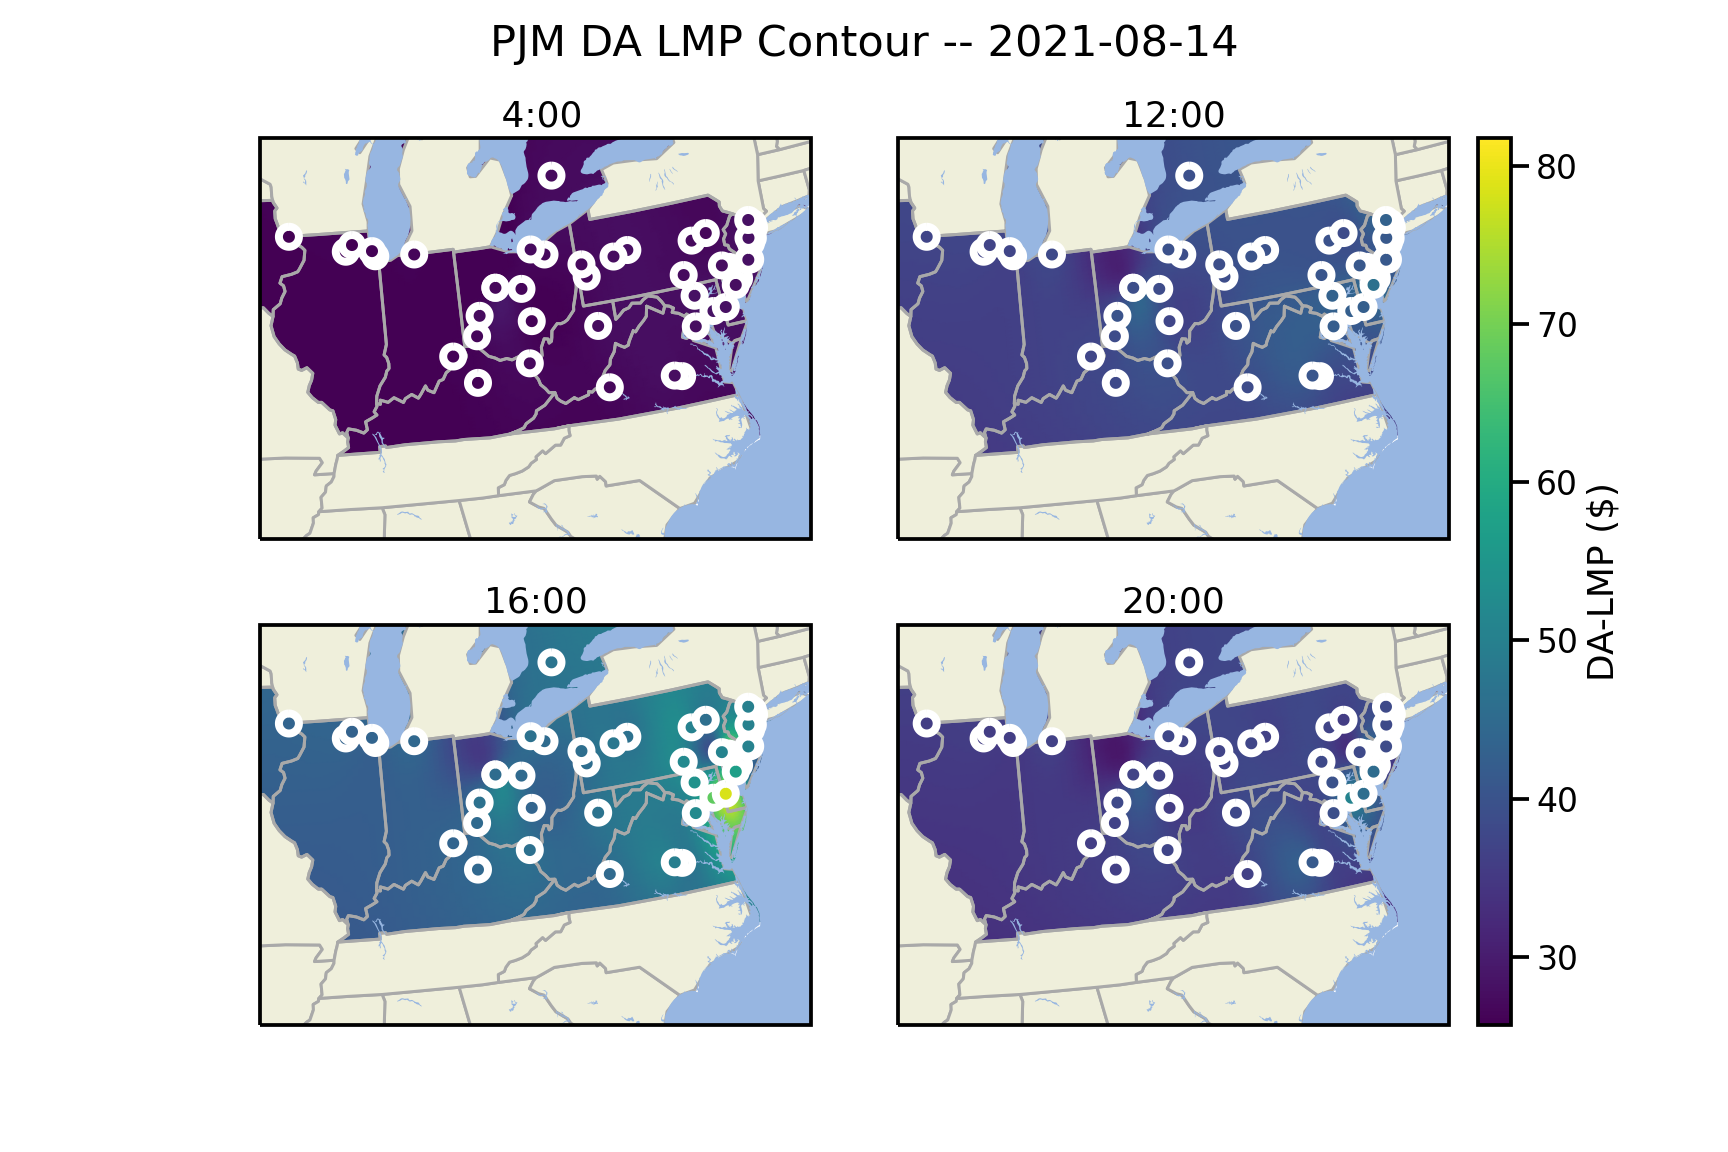
\includegraphics[width=150mm]{figs/pjm_lmp_contour_singlecbar}
%        }
    \end{center}
    \label{fig:contours}
\end{figure}

\section{The Application of Machine Learning to Energy Price Forecasting}\label{sec:the-application-of-machine-learning-to-price-forecasting}

The complicated task of forecasting nodal LMPs play a crucial role in the functioning of DA markets.
Accurate forecasts allow market participants to make informed trading decisions, plan generation and demand schedules,
and manage risk exposure.
Thus, poor forecasts can result in reduced market efficiency, realized as wasted generation resources, high energy
prices, and potentially greater carbon emissions~\cite{Surana2019}.
Factors such as volatile renewable generation, weather patterns, fuel prices, demand uncertainty, and complex
interactions between grid components make it a formidable challenge.
However, recent developments in machine learning, in particular deep learning methods, and access to historical market
data show promise at capturing the complex and dynamic structures essential for accurate forecasts.

\section{Motivation and Contributions}\label{sec:motivation}

We motivate the development of probabilistic forecasting methods by first discussing the limitations of common
point or interval forecasts.
Point forecasts, despite common usage, provide the least amount of information for decision-makers to act upon, as
all uncertainty is discarded to obtain a single value.
In comparison, interval forecasts, when paired with point forecasts, are substantially more informative.
The uncertainty surrounding a point forecast can often be captured as a confidence interval (CI), i.e. a range of
estimates which likely contain the ``true'' value for some confidence level.
The size of an interval can give decision-makers insight into the uncertainty of the forecast as ``wider'' CIs indicate
more uncertain forecasts.
Depending on the interpretations of the forecasts, the relationship between a combination of point and interval
forecasts can also provide insight into the uncertainty structure.
For example, a point estimate of the mean forecast near the bounds of an interval forecast may indicate certain
skewness and tail behavior of the underlying forecast uncertainty.
However, interval forecasts still discard valuable structural information such as multi-modality and tail behavior
outside the interval range.

Capturing all complexities and nuances of forecast uncertainty can only be achieved with probability density forecasts,
whereby a probability density function is defined over the entire forecast domain.
Despite powerful methods existing for low-dimensional problems, efficiently modeling joint conditional
distributions in high dimensions has long been extremely difficult.
Recent advances in deep neural-network-based generative models, in particular, \textit{normalizing flows}, show promise
for characterizing high dimensional and complex joint conditional probability densities.
Furthermore, certain constructions of normalizing flows allow both exact likelihood evaluation and efficient sampling,
which can enable powerful Monte Carlo methods to estimate key quantities of interest needed to make informed financial
decisions in energy markets.

In this work, we present a novel methodology for characterizing joint conditional probabilistic DA LMP
forecasts using normalizing flow generative models which can accurately capture conditional relationships
between market fundamentals and resulting prices, complex spatial correlations between price nodes, and forecast
uncertainty.
Additionally, we investigate several techniques to improve forecasting skill against non-stationary market data and the
use of generative adversarial network methods to refine performance in sampling-based tasks.
We also compare the forecasting performance of our proposed methods against point forecasting open-access benchmarks
from literature and a commercial optimal powerflow point forecasting product, demonstrating more
accurate forecasts than comparable solutions with unmatched uncertainty quantification.

The rest of this work is structured as follows.
In Chapter~\ref{ch:background} we outline the key mathematical background required to formulate probabilistic forecasts
using recent advances in deep generative modeling.
In Chapter~\ref{ch:methodology} we define our proposed methodology for characterizing probability density estimators
and generating probabilistic forecasts.
In Chapter~\ref{ch:experiments} we investigate techniques to improve forecasting skill in day-ahead energy markets and
compare our proposed methods against open-access benchmarks in energy price forecasting literature and commercial price
forecasting tools.
Finally, in Chapter~\ref{ch:conclusion} we summarize our key findings and lay out key future research paths to improve
model results, robustness, interpretability, and generalizability.

\section{Related Work}\label{sec:related-work}

Energy price forecasting literature can be split roughly into three categories: \textit{system pattern} (SP)
methods, statistical and machine learning methods, and deep-learning methods.

The work of Zhou et al.~\cite{5741753} develop the idea of SPs as an exploitation in the structure of the LMP optimization
problem formulation, where predictable market characteristics and associated \textit{system pattern regions} (SPRs), or
continuous neighborhoods of market conditions represented by polytopes in load space, give rise to specific predictable SPs.
Forecasting price action is then reduced to estimating which SPRs future market conditions will map to, and subsequently
retrieving the likely SPs and price action.
To overcome bias in the set of observed market states, a ``probabilistic'' formulation is also presented that can report
upper and lower quantile forecasts along with a mean forecast.
However, the SPR state space suffers from the curse of dimensionality, making analysis of large grids computationally
intractable.
Geng et al.~\cite{7478156} build upon the SPR concept, showing that they can be constructed using data-driven
methods, in particular learning SPR classification boundaries with support vector machines.
These data-driven SPR techniques are, however, still computationally intractable for anything more than small, synthetic
grid examples.
Radovanovic et al.~\cite{8733097} expand upon a similar idea to SPRs.
Through the use of recent advances in compressed sensing they reconstruct grid topologies allowing downstream inference
and clustering of congestion prices.
Clusters of generation-mix and load forecast are mapped to price clusters allowing for LMP forecasting.
The SPR-like representations make this method significantly more scalable for inference, however, training
the model incurs a costly step of reconstructing grid topology which can be significant for large grids~\cite{7226869}.

Using traditional statistical methods and machine learning methods, Uniejewski et al.~\cite{en9080621} propose a linear
auto-regressive model using ordinary least squares regression and LASSO automatic feature selection techniques.
This linear model can be modified for quantile regression tasks~\cite{UNIEJEWSKI2021105121} or with advanced
jump-diffusion and time-series techniques to produce probabilistic forecasts~\cite{MUNIAIN20201193}.
Andrade et al.~\cite{00000} present a methodology for both point and quantile forecasts using robust gradient boosting
trees and linear quantile regression, coupled with post-processing that exploits daily average prices to increase
forecast quality.

Deep-learning methods have recently risen in popularity for energy forecasting, beginning with the work of
Wang et al.~\cite{7744689} who present a stacked de-noising auto-encoder (SDA) neural network with unsupervised
pre-training and supervised fine-tuning regimes to improve forecast accuracy.
Subsequent work by Lago et al.~\cite{LAGO2018386} compare novel deep feed-forward neural network (DNN),
convolution neural network (CNN), and recurrent neural network (RNN) architectures and demonstrate the superiority of
deep-learning methods over traditional statistical methods.
A two-stage convolutional long short term memory (CLSTM) neural network to first
forecast generation bid curves to improve second-stage LMP point forecasts is proposed in~\cite{9916722}.
Zhang et al.~\cite{9520248} introduce a generative adversarial network (GAN) using a novel 3d tensor structure and
convolutional neural network to learn the spatiotemporal interactions from the tensor representation.
Cramer et al.~\cite{48550} develop a normalizing flows model to capture the joint probability distribution of multi-hour
price action on a single node and generate probabilistic forecasts for intra-day nodal prices in the German EPEX spot
market.
